% \documentclass[12pt]{template}
% \usepackage{fancyhdr}

% \begin{document}   
\section{事件描述对事件参与人数的影响} 
\subsection{背景介绍}  
  近年来,社交平台的出现极大的方便的人们的生活。在其中一些平台上,人们可以发布事件,
参与事件。这类平台上的社交网络与传统的社交网络有着很大的不同,例如网络中的参与者,除了
在线上有着联系,在线下也互相接触,以及网络中的内容具有时效性等等。为了将其与传统的社交
网络区分开来,学者提出了\textbf{基于事件的社交网络}(\textbf{EBSN})\cite{EBSN_linking}。它将社交网络分为线上和线下两个部分:线上部分与传统社交网络类似,而人们参与同一事件的记录则保存在线下部分。
 
为了能吸引更多的用户参与事件,事件组织者需要尽可能的使自己组织的事件在同类事件中
有更高的吸引力,而一份问题描述在提高事件吸引力上所起的作用是相当显著的。例如下面
两段事件描述,从直觉上来说,第一段描述显然比第二段更有活力。而事实也是如此,第一
个事件的参与人数(超过97\%的同类事件)要远高于后者(超过5\%的同类事件)。
 
\begin{quotation}
  \textit{let  \'s get ready to get in our bikinis and board shorts  (  spe
  edos for the europeans  )  and enjoy the la summer heat on the beach
  !  this year the event is on saturday  ,  august 10th starting at 
  1pm . we will have muchies  ,  drinks and games . for those that 
  are into volleyball  ,  let  \'s repeat what we did last year . 
  i saw a lot of losers  ,  i mean winners. lol . let  \'s enjoy 
  a few good volleyball game . \\ 
  }
    
  \textit{open to the public for a group class package and individual classes}
\end{quotation}

接下来的结构如下:在第二节,我们会定义问题并建立模型,第三节会对描述文本建模,
并使用拉索回归来寻找对事件成功起关键性的词,第四节则介绍了事件相似矩阵的定义,第五
节则用实验来证明文本质量会对事件成功产生影响。

\subsection{问题描述}
\subsubsection{数据集}

meetup\footnote{http://www.meetup.com/about}是一家提供在线组织活动的平台,
在meetup上,一个用户可以根据自己的兴趣加入不同的小组\(G\),并在
组内参与或发布事件。有些小组内的活动仅开放给组员参加,有些则对公众
开放。我们爬取了meetup在LA的部分数据,包括当地的组,组内成员信息
及组的历史事件。具体信息如表(\ref{t1})。

\begin{longtable}[HTBP]{@{}lc@{}}
\toprule
& LA\tabularnewline
\midrule
\endhead
Users & 172673\tabularnewline
Events & 166829\tabularnewline
Groups & 2507\tabularnewline
\bottomrule
\caption{}
\label{t1}
\end{longtable}

我们使用一个七元组来表示一个事件\(e_{id}(id,t,d,h,a,l,c)\),其中\(t\)是事件举办时间,\(d\)是事件描述,\(h\)是事件所在组,\(a\)是事件参与人,\(l\)是事件所在地点。\(c\)是事件主题:meetup的事件有36个主题。以及三元组来表示组\(g_{id}(id,e,m,c)\),其中\(e\)是事件,\(m\)是组内成员,\(c\)是该组的主题。

\subsection{问题定义}
\textbf{定义一: 成功事件}指对于一个事件\(e_{id}\)和与其相似的事件\(E\{e_1,e_2,e_3,...\}\),
\(|e_{id}^a|\)大于\(E\)中\(70\)\%的事件。

衡量事件成功的因素有很多,这里使用了一个比较客观的信息:参与人数。因为对绝大多数事件举办者来说,如果事件参与人数超过了同类事件的百分之七十五,那么该事件可以算得上是成功事件了。

\textbf{定义二: 相同事件}指对于事件\(e_{id_1}\)和事件\(e_{id_2}\),\(e_{id_1}^d=e_{id_2}^d\)

在meetup中有大约30\%的事件属于相同事件,它们对于推荐算法意义重大,但如果只为了考察事件描述对事件成功的影响,则会起到相反的作用。因为在衡量事件描述产生的影响时,该类事件会增加其事件描述的影响比重,进而导致结果偏向于重复出现的事件描述。其二是参与这类事件的人有着很大的重叠,他们是基于经历而不是基于事件描述来选择参与该事件的,所以他们对事件描述不敏感。因此剔除该类事件是有必要的。对于相同事件,我们只保留其中出现时间最早的。

\textbf{定义三: 相似事件}
指对于事件\(e_{id_1}\)和事件\(e_{id_2}\),\(sim(e_{id_1},e_{id_2})>\gamma\),其中\(sim\)是相似矩阵,\(\gamma\)是阈值。关于相似矩阵建立和阈值的选择可以在第\ref{4}节看到。

根据以上的三个定义,最终的问题定义如下:

\textbf{定义四: 问题定义}

给定事件\(e_{id}\)和相似事件\(E\{e_1,e_2,...\}\),判断\(|e_{id}^a|\)
是否超过了\(E\)中70\%的事件。由此可见,我们把该问题转化成了一个预测问题。

\subsection{文本建模}

\subsubsection{拉索回归}

拉索回归是线性回归的一种,它可以通过系数的大小选出重要的变量\cite{tibshirani_regression_1996},因此我们可以对参与人数进行回归,来挑选出对参与人数影响比较大的单词\cite{noauthor_predicting_nodate}。

\[
argmin\left\{\displaystyle\sum_{i=1}^N\left(y_i-\beta_0-\displaystyle\sum_j\beta_jx_{ij}\right)\right\}
\] \[subject\ to \displaystyle\sum_j|\beta_j|\leq\alpha\]\\

其中\(y_i\)为第\(i\)个目标即参与人数,\(x_{ij}\)为\(e_i^d\)中第\(j\)个单词。\(\alpha,\beta_0\)为预先设定的参数。
\subsection{文本处理}\label{3.2}

这里我们使用独热编码(one hot)对文本建模,并去除停止词和非英文单词。然后使用
交叉验证和网格搜索来确定拉索回归的最佳参数。我们希望使用拉索回归来寻找对参与人数影响最大的
单词,并得到一个可以解释的结果。在这次实验中,我们随机挑选了100个组,其中包含了8673个事件,去除相同
事件后还剩5579个事件。将这些事件的事件描述作为输入,对它们的参与人数进行回归后挑选出了
系数最高和最低的8个词,如表(\ref{t2})所示:

\begin{longtable}[HTBP]{@{}lc@{}}
\toprule
系数最高的8个词 & 系数最低的8个词\tabularnewline
\midrule
\endhead
christmas & week\tabularnewline
dance & saga\tabularnewline
directions & meditation\tabularnewline
cocktails & information\tabularnewline
concerts & salt\tabularnewline
band & mammoth\tabularnewline
perfect & spiritual\tabularnewline
tribute & masked\tabularnewline
drinks & learn\tabularnewline
\bottomrule
\caption{}
\label{t2}
\end{longtable}
  
其中有些词符合人的主观判断,例如cocktails,drinks等,有些则不那么直观,比如spiritual(这个词出现在一个教堂组织的礼拜活动中),不过这个实验结果从某些程度上印证了我们的猜想:在聚会活动中,一起开party显然比一起做礼拜要有吸引力。当然其中也有些无法解释的词,这是由于拉索回归的局限和样本太少导致的。

然而简单的对所有事件做回归是一种不公平的做法,因为有些种类的活动,例如喝下午茶,其参与人数和另一些活动例如踢足球,有着先天的区别。因此有必要将不同的事件分开来,让比较仅在相似的事件间进行。因此,如何找到相似的事件便变得重要了。在接下来的一节,我们将给出一系列相似矩阵的定义,从而最终得到事件的相似矩阵。

\subsection{事件相似度}
由meetup上爬取的数据来看,一个事件由时间,地点,主题,举办者,举办组等属性决定,因此,我们可以通过定义这些属性的相似度来反推事件的相似度。

\subsubsection{举办组的相似度}
两个组的相似可以分为两个方面,一是组的主题相似,二是组的成员相似。分别的,我们对应定义了两个矩阵:

\textbf{(1) 主题相似度} \(group\_cat\_sim:\)

\[
group\_cat\_sim(i,j)=\frac{|g_i^c\bigcap g_j^c|}{|g_i^c|}
\]

\textbf{(2) 成员相似度} \(group\_mem\_sim:\)

\[
group\_mem\_sim(i,j)=\frac{|g_i^m\bigcap g_j^m|}{|g_i^m|}
\]

通过这两个矩阵的线性组合,我们就能衡量出两个组间的相似度。

\subsubsection{事件主题相似度}

和组主题相似度类似,定义如下:

\[
event\_cat\_sim(i,j)=\frac{|e_i^c\bigcap e_j^c|}{|e_i^c|}
\]

\subsubsection{时间相似度}

我们希望相似的事件在时间上也更接近,时间相似度越大。同时我们也希望确保时间相似度的值域能在\([0,1)\)之间,因此,使用负指数函数。

\[    
time\_sim(i,j)=\mathrm{e}^\frac{-|e_i^t-e_j^t|}{\alpha}
\]

其中\(\alpha\)为参数。

\subsubsection{地点相似度}

同样的,距离越近的事件地点相似度越高。这里使用haversine公式计算出两点之间的距离

\[    
loc\_sim(i,j)=\mathrm{e}^\frac{-|e_i^l-e_j^l|}{\alpha}
\]

\subsubsection{事件相似度}
基于以上5个矩阵,我们定义如下事件相似矩阵:

\[    
event\_sim(i,j)=\alpha*group\_mem\_sim+\beta*group\_cat\_sim
+{c}*time\_sim+{d}*loc\_sim+{e}*event\_cat\_sim
\]

其中\(\{\alpha,\beta,{c},{d},{e}\}\)都是归一化后的参数,
至于阈值\(\gamma\)的选择则应该参考\(event\_sim\)的值的分布,在实验中我们使用了前20\%的数值。

\subsection{实验结果}

\subsubsection{实验设计}
为了考察事件描述对事件成功的影响,我们设计了如下实验:首先,使用第\ref{4}节定义的\(event\_sim\)选出相似的事件。然后根据事件成功的定义,对事件进行标注,然后使用事件训练分类器,比较包含事件描述和不包含事件描述对分类结果的影响。最后,建立关于参与人数的混合模型,并将事件描述作为可选项,比较包含和不包含事件描述对\(R^2\)的影响。
本次实验的数据为之前爬取的LA数据。

\subsubsection{计算事件相似度}
我们根据之前第四节提出的方法计算出了\(event\_sim\)矩阵,其中\(\{\alpha,\beta,{c},{d},{e}\}\)分别为\(\{\frac{1}{8},\frac{1}{8},\frac{1}{4},\frac{1}{4},\frac{1}{4}\}\)。得到的相似矩阵热力图(图(\ref{ff1}))和值的分布(图(\ref{ff2}))。

\begin{figure}[htbp]
  \centering
  \begin{minipage}[t]{0.48\textwidth}
  \centering
  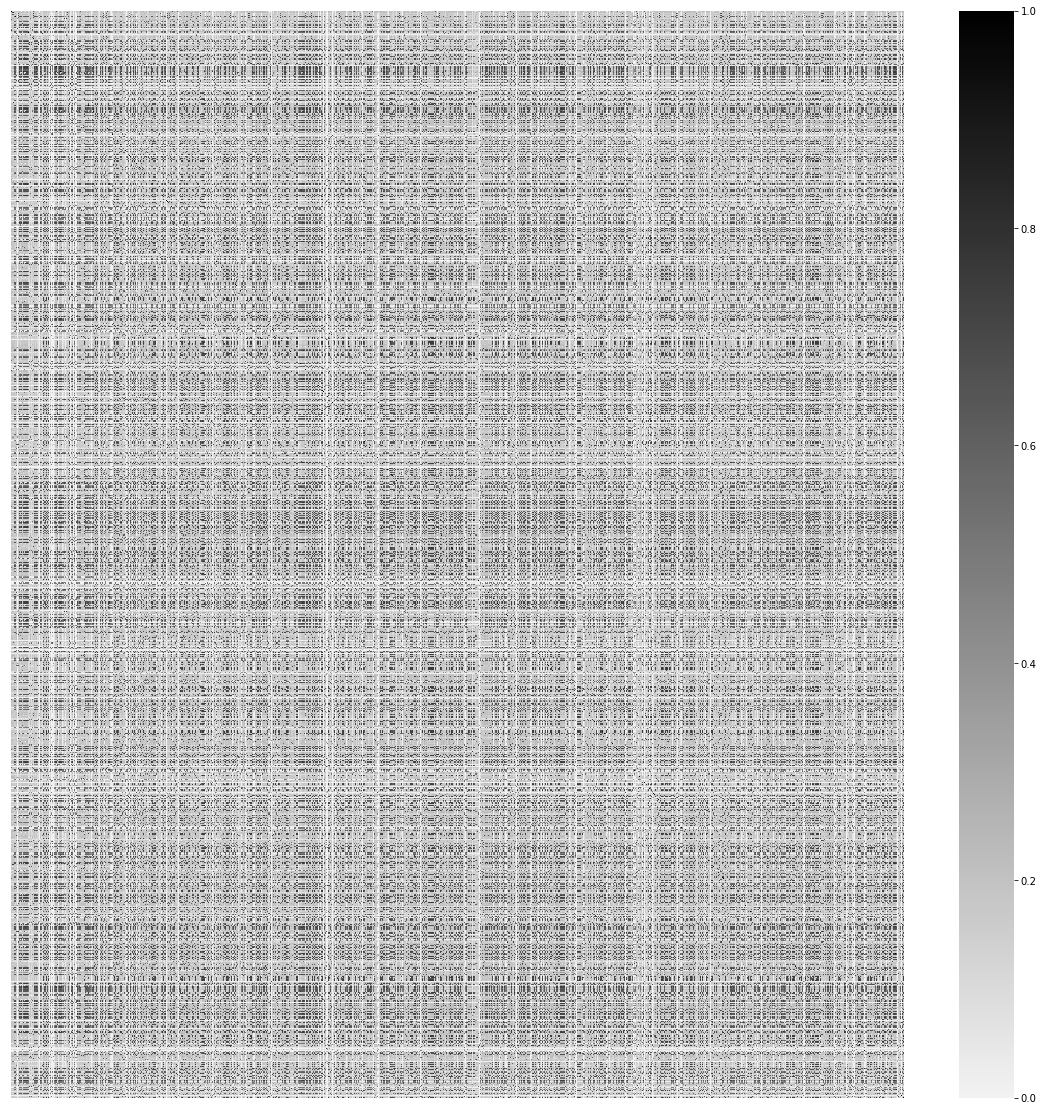
\includegraphics[width=6cm]{event_sim.png}
  \caption{热力图}
  \label{ff1}
  \end{minipage}
  \begin{minipage}[t]{0.48\textwidth}
  \centering
  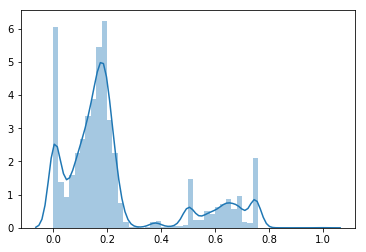
\includegraphics[width=6cm]{event_sim_dist.png}
  \caption{分布}
  \label{ff2}
  \end{minipage}
\end{figure}

可以看出相似矩阵值在0.5附近有较大的差异,因此我们把阈值取为0.5。然后我们通过事件成功的定义来对所有事件的成功性进行标注。

\subsubsection{训练分类器}
为了初步的衡量事件的描述对事件参与人数的影响,我们可以将描述作为一个可选的属性,使用一些常用的分类器,例如随机森林,adaboast,对事件成功性进行预测。这里输入是向量化后事件的属性,输出是之前的标注结果。为了避免稀疏高维的文本向量对分类效果的影响,这里对文本的处理方式参考了第二节所用的方法,即事先训练好一个拉索回归器,使用该回归器产生的值来取代原始文本。这里使用拉索回归仅是为了方便,仅针对文本应该有更好的处理方式。

最终我们使用adaboost,决策树,knn和随机森林作为分类器,使用4折交叉验证来衡量结果,使用网格搜索来确定最佳参数。
本次实验平台为i5-4200m,内存为8G,显卡为gtx-730m。实验结果如图(\ref{f3}):

\begin{figure}
\centering
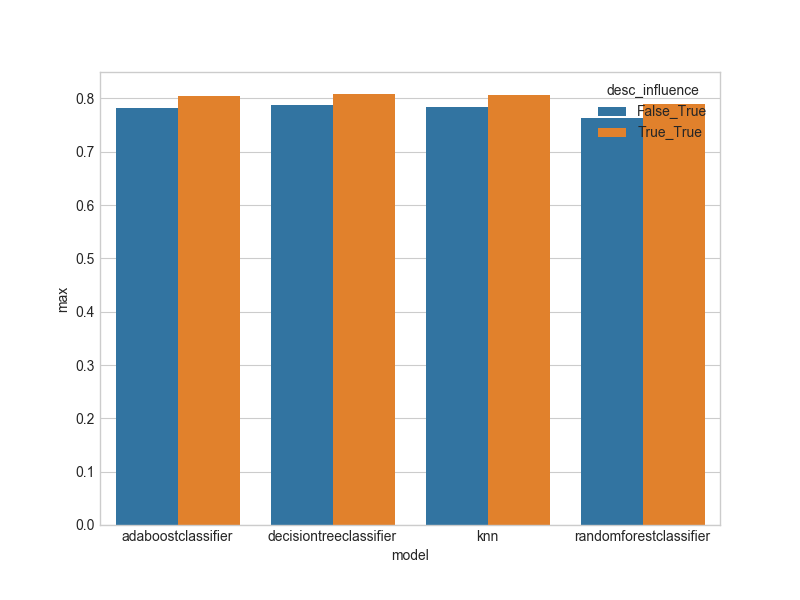
\includegraphics[width=10cm]{exp4_with_1.png}
\caption{}
\label{f3}
\end{figure}

通过实验结果可以看出,加入了事件描述后,分类的精度有了提高。注意到这里排除了相同事件,所以提高的原因不是因为相同事件之间参与人数的相似性。由此可以得出结论:事件描述对预测事件成功起正面作用。不过提高有限,这是由于多种原因造成的:一是由于文本处理的方式过于粗糙,二是由于样本太少(交叉验证时每次训练量大概只有3000条),三是由于样本分布不均匀(大概75\%的事件是负样本)。

\subsubsection{建立混合模型}

为了能更进一步的说明事件描述的加入提高了模型的解释能力,我们使用了混合模型对参与人数与事件的属性之间的关系进行描述。注意到这里我们并不是想根据事件去推算参与人数,而是想给予此判断事件描述在整个模型中起的作用。我们建立的混合模型如下:

\[
y_{ijkm}=\beta_0+log|g_i^m|+\gamma_j+\alpha_k+ (\phi_m) +\epsilon_{ijkm}
\]

其中\(\gamma_j\),\(\alpha_k\)和\(\phi_m\)为事件主题,事件举办人和事件描述的随机效应,固定效应为组内人数。

Nakagawa和Schielzeth\cite{nakagawa_ageneralandsimplemethodforobtaining_2013}提出了衡量混合模型中的确定系数\(R^2\),在混合模型中,确定系数分为两种,一是\(R_m^2\),衡量固定效应对模型的作用,二是\(R_c^2\),衡量所有效应对模型的作用。计算方法如下:

\[
R_m^2=\frac{\sigma_m^2}{\sigma_m^2+\sigma_\gamma^2+\sigma_\alpha^2+(\sigma_\phi^2)+\alpha_\epsilon^2}
\] \[
R_c^2=\frac{\sigma_m^2+\sigma_\gamma^2+\sigma_\alpha^2+(\sigma_\phi^2)}{\sigma_m^2+\sigma_\gamma^2+\sigma_\alpha^2+(\sigma_\phi^2)+\alpha_\epsilon^2}
\]

其中\(\sigma\)为方差。混合模型使用了R语言中的``lme4''计算包\cite{lme4},\(R^2\)的计算使用了R语言
中的``MuMIn''计算包\cite{MuMIn}。结果如表(\ref{t3})。

\begin{table}[htbp]
	\centering
  \caption{}
  \label{t3}
	\begin{tabular}{cll}
		\hline
                           &  \(R_c^2\) & \(R_m^2\) \\ 
    \hline
		包含事件描述                       & \textbf{0.653} & 0.135 \\ 
    不包事件含描述                        & 0.494 & 0.135 \\ 
    \hline
	\end{tabular}
\end{table}

可以看出包含事件描述后,\(R_c^2\)显著提高,模型的解释性得到了加强。另一个值得注意的是组的规模对事件参与人数并没有特别显著的影响。

\subsection{小结}
本文定义了事件相似性,并使用拉索回归对事件描述进行回归,得到了可解释的结果。然后使用一系列分类器证明了事件描述可以帮助预测事件成功性,最后使用了混合模型证明了该提升并不只是增加了多余的信息,而是提高了模型的解释能力,由此得出事件描述是影响事件是否成功的非常重要的一环的结论。

然而,值得注意的是,本文并没能回答什么样的事件描述会促使事件的成功。虽然从拉索回归得到的系数能衡量不同词语对事件成功的影响的重要程度,但这仍只是归纳而非推理。而从已有的事件描述总结出好的事件描述的规律,并以此生成其他事件描述将是更有意义的工作,这将留待以后来完成。

% \end{document}